\documentclass[12pt]{sty/colt2019/colt2018-arxiv}
% \else
% \documentclass[anon,12pt]{sty/colt2019/colt2019} % Anonymized submission
% \documentclass[12pt]{colt2019} % Include author names
% \fi

% The following packages will be automatically loaded:
% amsmath, amssymb, natbib, graphicx, url, algorithm2e

% \title[Short Title]{Full Title of Article}
\title{Implicit regularization in DPP subset selection}
\usepackage{times}
 
\usepackage{color}
\usepackage{cancel}
\usepackage{wrapfig}
\usepackage{caption}
\usepackage{algorithm}
\usepackage{xfrac}
\usepackage{algorithmic}
\def\opt{{\textsc{OPT}_k}}
\def\const{{\mathrm{const}}}
\def\nnz{{\mathrm{nnz}}}
\def\r{\sfrac{\sigma_{\w}^2}{\sigma_{\xib}^2}}
\def\rm{\sfrac{\sigma_{\xib}^2}{\sigma_{\w}^2}}
\def\cmark{\Green{\checkmark}}
\def\xmark{\Red{\large\sffamily x}}
\newcommand{\pdet}{{\mathrm{pdet}}}
\newcommand{\MSPE}[1] {{\mathrm{MSPE}\big[#1\big]}}
\newcommand{\MSE}[1] {{\mathrm{MSE}\big[#1\big]}}
\def\Poisson{{\operatorname{Poisson}}}
\def\PB{{\operatorname{PB}}}
\newcommand{\DP}[1]{\mathcal{DP}^{#1}}
\def\Ic{\mathcal{I}}
\def\Jc{\mathcal{J}}
\def\Mc{\mathcal M}
\def\Ec{\mathcal E}
\def\sr{{\mathrm{sr}}}
\def\ktd{{k^{\underline{d}}}}
\def\Det{{\mathrm{Det}}}
\def\detu{{\widecheck{\mathrm{Det}}_\mu^\gamma}}
\def\deto{{\widehat{\mathrm{Det}}_\mu^\gamma}}
\def\Zu{{\widecheck{Z}_\mu^{\gamma}}}
\def\Zo{{\widehat{Z}_\mu^{\gamma}}}
\def\Zun{{\widecheck{Z}_\mu^{\gamma_n}}}
\def\Zon{{\widehat{Z}_\mu^{\gamma_n}}}
\newcommand{\Er}{\mathrm{Er}}
\newif\ifDRAFT
\DRAFTtrue
\ifDRAFT
\newcommand{\marrow}{\marginpar[\hfill$\longrightarrow$]{$\longleftarrow$}}
\newcommand{\niceremark}[3]
   {\textcolor{red}{\textsc{#1 #2:} \marrow\textsf{#3}}}
\newcommand{\ken}[2][says]{\niceremark{Ken}{#1}{#2}}
\newcommand{\manfred}[2][says]{\niceremark{Manfred}{#1}{#2}}
\newcommand{\michael}[2][says]{\niceremark{Michael}{#1}{#2}}
\newcommand{\michal}[2][says]{\niceremark{Michal}{#1}{#2}}
\newcommand{\feynman}[2][says]{\niceremark{Feynman}{#1}{#2}}
%\usepackage[inline]{showlabels}
\else
\newcommand{\ken}[1]{}
\newcommand{\michael}[1]{}
\newcommand{\michal}[1]{}
\newcommand{\feynman}[1]{}
\fi
\newcommand{\norm}[1]{{\| #1 \|}}

\newcommand{\deff}{d_{\textnormal{eff}}}
\def\ee{\mathrm{e}}
\newcommand\mydots{\makebox[1em][c]{.\hfil.\hfil.}}
\def\Sd{\mathscr{S}_{\!d}}
\newcommand{\dx}{\dxy_{\!\cal X}}
\newcommand{\dxk}{\dxy_{\!\cal X}^k}
\newcommand{\dk}{\dxy^k}
\newcommand{\dxy}{\mathrm{D}}
\def\simiid{\overset{\textnormal{\fontsize{6}{6}\selectfont
i.i.d.}}{\sim}}
%\newcommand{\Dxy}{D_{\!\cal X\!,\cal Y}}
\def\vskx{{\mathrm{VS}_{\!\dx}^k}}
\def\vsk{{\mathrm{VS}_{\!D}^k}}
\def\vskxm{{\mathrm{VS}_{\!\dx}^{k-1}}}
\def\vskm{{\mathrm{VS}_{\!D}^{k-1}}}
\def\vsdx{{\mathrm{VS}_{\!\dx}^d}}
\def\vsd{{\mathrm{VS}_{\!D}^d}}
\newcommand{\vs}[1]{{\mathrm{VS}_{\!D}^{#1}}}
\newcommand{\sigd}{\boldsymbol\Sigma_{\!\dx}}
\def\wols{\w_{\mathrm{LS}}}
\def\wds{\boldsymbol\w_{\!D}^*}
\def\kd{K_{\!\dx}}

\def\poly{{\mathrm{poly}}}
\def\polylog{{\mathrm{polylog}}}
\def\DPP{{\mathrm{DPP}}}
\def\DPPcor{{\DPP_{\!\mathrm{cor}}}}
\def\DPPens{{\DPP_{\!\mathrm{ens}}}}
\newcommand{\DPPreg}[1]{{\DPP_{\!\mathrm{reg}}^{#1}}}
\def\Vol{{\mathrm{VS}}}
\def\Lev{{\mathrm{Lev}}}
\newcommand\todod[1]{\Red{\# DH: #1}}
\newcommand{\explain}[2]{\mathrel{\overset{\makebox[0pt]{\text{\tiny
#1}}}{#2}}}
\def\tot {{\mathrm{tot}}}
\def\checkmark{\tikz\fill[scale=0.4](0,.35) -- (.25,0) --
(1,.7) -- (.25,.15) -- cycle;}
\newcommand{\mnote}[1]{{\bf\large \Magenta{*}}\marginpar{\small \Magenta{#1}}}
\newcommand{\bnote}[1]{{\bf #1}}

\newcommand{\sqrtshort}[1]{{\sqrt{\white{\Big|}\!\!\smash{\text{\fontsize{9}{9}\selectfont$#1$}}}}}
\newenvironment{proofof}[2]{\par\vspace{2mm}\noindent\textbf{Proof of {#1} {#2}}\ }{\hfill\BlackBox}
\newcommand{\sets}[2]
{{\hspace{-0.3mm}[\hspace{-0.3mm}#1\hspace{-0.3mm}]\hspace{-0.3mm}\choose
\hspace{-0.3mm}#2\hspace{-0.3mm}}}
\DeclareMathOperator{\sgn}{\textnormal{sgn}}
\DeclareMathOperator{\adj}{\textnormal{adj}}
\def\Rb{{\mathbf{R}}}
\DeclareMathOperator{\ws}{\widetilde{\w}}
\newcommand{\inote}[1]{{\bf {#1}}}
\def\xib{\boldsymbol\xi}
\def\Sigmab{\mathbf{\Sigma}}
\def\Sigmabh{\widehat{\Sigmab}}
\def\Sigmabt{\widetilde{\Sigmab}}
\def\S{\mathbf{S}}
\def\T{\mathbf{T}}
\def\xt{\tilde{x}}
\def\xbt{\widetilde{\x}}
\def\xbh{\widehat{\x}}
\def\ubh{\widehat{\u}}
\def\dom {{\mathrm{dom}}}
\def\val {{\mathrm{val}}}
\def\out {{\mathrm{out}}}
\def\iin  {{\mathrm{iin}}}
\def\s {\mathbf{s}}
\def\q {\mathbf{q}}
\def\qt{\tilde{q}}
\def\itld {j}
\def\ubt {\tilde{\u}}
\def\n{\{1..n\}}
\def\cb {\mathbf{c}}
\def\cW{\mathcal W}
\def\Xt{\widetilde{X}}
\def\Dbt{\widetilde{\D}}
\def\xtb{\tilde{\mathbf{x}}}
\def\ytb{\tilde{\mathbf{y}}}
\def\Xtb{\widetilde{\mathbf{X}}}
\def\Xbb{\overline{\X}}
\def\Xb{{\bar{\X}}}
\def\ybb{\overline{\y}}
\def\f{{\mathbf{f}}}
\def\g{{\mathbf{g}}}
\def\fbb{{\overline{\f}}}
\def\fb{{\overline{f}}}
\def\Xc{\mathcal{X}}
\def\W{\mathbf W}
\def\L{\mathbf{L}}
\def\Rb{\mathbf R}
\def\Pc{\mathcal{P}}
\def\Nc{\mathcal{N}}
\def\Pt{\widetilde{P}}
\def\Hc{\mathcal{H}}
\def\Wc{\mathcal{W}}
\def\Cc{\mathcal{C}}
\def\p{\mathbf p}
%\def\r{\mathbf r}
\def\Y{\mathbf Y}
\def\H{\mathbf H}
\def\K{\mathbf K}
\def\Kh{\widehat{K}}
\def\Kbh{{\widehat{\K}}}
\def\Q{\mathbf Q}
\def\Qbar{{\bar{\mathbf Q}}}
\def\Ytb{\widetilde{\mathbf{Y}}}
\def\c{{n-d\choose s-d}}
\DeclareMathOperator{\Proj}{Proj}
\newcommand{\Span}{\mathrm{span}}
\newcommand{\ofsubt}[1]{\mbox{\scriptsize \raisebox{0.25pt}{$(#1)$}}}
%\raisebox{0.5pt}{$($}}#1\mbox{\tiny \raisebox{0.5pt}{$)$}}}
\newcommand{\ofsub}[1]{\mbox{\small \raisebox{0.0pt}{$(#1)$}}}
%\newcommand{\ofsubb}[1]{\mbox{\footnotesize \raisebox{0.5pt}{$(#1)$}}}
%\newcommand{\ofsub}[1]{(#1)}
%\newcommand{\ofsub}[1]{\mbox{\tiny$|$\hspace{-0.5pt}\raisebox{-0.5pt}{$#1$}}}
\newcommand{\of}[2]{{#1{\!\ofsub{#2}}}}
\newcommand{\oft}[2]{{#1{\!\ofsubt{#2}}}}
\newcommand{\fof}[2]{{#1({#2})}}
\newcommand{\yof}[2]{{#1{\ofsub{#2}}}}
%\newcommand{\yofb}[2]{{#1{\ofsubb{#2}}}}
\newcommand{\lazy}{FastRegVol}
\newcommand{\volsamp}{RegVol}

\newcommand{\Sm}{{S_{-i}}}
\newcommand{\Sp}{{S_{+i}}}
\ifx\BlackBox\undefined
\newcommand{\BlackBox}{\rule{1.5ex}{1.5ex}}  % end of proof
\fi
%\renewcommand{\dagger}{+}
\DeclareMathOperator*{\argmin}{\mathop{\mathrm{argmin}}}
\DeclareMathOperator*{\argmax}{\mathop{\mathrm{argmax}}}
\DeclareMathOperator*{\diag}{\mathop{\mathrm{diag}}}
\def\x{\mathbf x}
\def\y{\mathbf y}
\def\ybh{\widehat{\mathbf y}}
\def\ybb{\bar{\mathbf y}}
\def\xbb{\bar{\mathbf x}}
\def\yb{{\bar y}}
\def\ybt{\widetilde{\mathbf y}}
\def\yh{\widehat{y}}
\def\yhb{\widehat{\y}}
\def\yt{\widetilde{y}}
\def\z{\mathbf z}
\def\a{\mathbf a}
\def\b{\mathbf b}
\def\w{\mathbf w}
\def\v{\mathbf v}
\def\m{\mathbf m}
\def\wbh{\widehat{\mathbf w}}
\def\wh{\widehat{\mathbf w}}
\def\vbh{\widehat{\mathbf v}}
\def\wbt{\widetilde{\mathbf w}}
\def\e{\mathbf e}
\def\zero{\mathbf 0}
\def\one{\mathbf 1}
\def\u{\mathbf u}
\def\ubbar{\bar{\mathbf u}}
\def\f{\mathbf f}
\def\ellb{\boldsymbol\ell}

\def\X{\mathbf X}
\def\Xs{\widetilde{\X}}
\def\B{\mathbf B}
\def\A{\mathbf A}
\def\C{\mathbf C}
\def\U{\mathbf U}
\def\Ubt{\widetilde{\mathbf U}}
\def\Ubh{\widehat{\mathbf U}}
\def\Ubbar{\bar{\mathbf U}}
\def\F{\mathbf F}
\def\D{\mathbf D}
\def\V{\mathbf V}
\def\M{\mathbf M}
\def\Mh{\widehat{\mathbf M}}
%\def\S{\mathbf S}
\def\Stb{\widetilde{\mathbf{S}}}
\def\Sbh{\widehat{\mathbf{S}}}
\def\St{\widetilde{\S}}
\def\Sh{\widehat{S}}
\def\Sc{\mathcal{S}}
\def\Fc{\mathcal{F}}
\def\Vc{\mathcal{V}}
\def\Bc{\mathcal{B}}
\def\Dc{\mathcal{D}}
\def\Z{\mathbf Z}
\def\Zbh{\widehat{\mathbf Z}}
\def\Zbt{\widetilde{\mathbf Z}}
\def\Abh{\widehat{\mathbf A}}
\def\I{\mathbf I}
\def\Ic{\mathcal I}
\def\II{\mathbf {I \!\,I}}
%\def\II{\boldsymbol {\mathbb I}}
\def\A{\mathbf A}
\def\P{\mathbf P}
\def\Ph{\widehat{\mathbf P}}
\def\cP{\mathcal P}
\def\cR{\mathcal R}
\def\Xt{\widetilde{\mathbf{X}}}
\def\Xh{\widehat{\mathbf{X}}}
\def\Rh{\widehat{R}}
\def\Ot{\widetilde{O}}
\def\At{\widetilde{\A}}


\def\E{\mathbb E}
\def\R{\mathbb R}
\def\N{\mathbb N}
\def\Pr{\mathrm{Pr}}
%\def\C{\mathbb C}
\def\tr{\mathrm{tr}}
\def\Sbar{{\bar{S}}}
\def\cS{{\mathcal{S}}}
\def\Tbar{{\bar{T}}}
\def\Tt{{\widetilde{T}}}
\def\rank{\mathrm{rank}}
\def\Prob{\mathrm{Prob}}
\def\Var{\mathrm{Var}}
\def\Xinv{(\X^\top\X)^{-1}}
\def\XinvS{(\X_S\X_S^\top)^{-1}}
\def\ABinvS{(\A_S\B_S^\top)^{-1}}
\def\ABinv{(\A\B^\top)^{-1}}
\def\xinv{\x_i^\top\Xinv\x_i}
\def\Xinvr{(\lambda\I+\X_{-1}^\top\X_{-1})^{-1}}
\def\pdet{\mathrm{pdet}}
\newcommand{\vol}{\mathrm{vol}}
%\newcommand{\defeq}{:=}
\newcommand{\defeq}{\stackrel{\textit{\tiny{def}}}{=}}
\newcommand{\di}{{[d+1]_{-i}}}
\newcommand{\cov}{\mathrm{cov}}
\let\origtop\top
\renewcommand\top{{\scriptscriptstyle{\origtop}}} % this makes transpose not so big

\definecolor{silver}{cmyk}{0,0,0,0.3}
\definecolor{yellow}{cmyk}{0,0,0.9,0.0}
\definecolor{reddishyellow}{cmyk}{0,0.22,1.0,0.0}
\definecolor{black}{cmyk}{0,0,0.0,1.0}
\definecolor{darkYellow}{cmyk}{0.2,0.4,1.0,0}
\definecolor{orange}{cmyk}{0.0,0.7,0.9,0}
\definecolor{darkSilver}{cmyk}{0,0,0,0.1}
\definecolor{grey}{cmyk}{0,0,0,0.5}
\definecolor{darkgreen}{cmyk}{0.6,0,0.8,0}
\newcommand{\Red}[1]{{\color{red}  {#1}}}
\newcommand{\Purple}[1]{{\color{purple}  {#1}}}
\newcommand{\Magenta}[1]{{\color{magenta}{#1}}}
\newcommand{\Green}[1]{{\color{darkgreen}  {#1}}}
\newcommand{\Blue}[1]{\color{blue}{#1}\color{black}}
\newcommand{\Orange}[1]{\textcolor{orange}{#1}\color{black}}
\newcommand{\Brown}[1]{{\color{brown}{#1}\color{black}}}
\newcommand{\Grey}[1]{{\color{grey}{#1}\color{black}}}
\newcommand{\white}[1]{{\textcolor{white}{#1}}}
\newcommand{\yellow}[1]{{\textcolor{reddishyellow}{#1}}}
\newcommand{\darkYellow}[1]{{\textcolor{darkYellow}{#1}}}
\newcommand{\grey}[1]{{\textcolor{grey}{#1}}}

\DeclareMathOperator{\half}{\frac{1}{2}}

\ifx\proof\undefined
\newenvironment{proof}{\par\noindent{\bf Proof\ }}{\hfill\BlackBox\\[2mm]}
\fi

\ifx\theorem\undefined
\newtheorem{theorem}{Theorem}
\fi

\ifx\example\undefined
\newtheorem{example}{Example}
\fi

\ifx\condition\undefined
\newtheorem{condition}{Condition}
\fi
\ifx\property\undefined
\newtheorem{property}{Property}
\fi

\ifx\lemma\undefined
\newtheorem{lemma}{Lemma}
\fi

\ifx\proposition\undefined
\newtheorem{proposition}{Proposition}
\fi

\ifx\remark\undefined
\newtheorem{remark}{Remark}
\fi

\ifx\corollary\undefined
\newtheorem{corollary}{Corollary}
\fi

\ifx\definition\undefined
\newtheorem{definition}{Definition}
\fi

\ifx\conjecture\undefined
\newtheorem{conjecture}{Conjecture}
\fi

\ifx\axiom\undefined
\newtheorem{axiom}{Axiom}
\fi

\ifx\claim\undefined
\newtheorem{claim}{Claim}
\fi

\ifx\assumption\undefined
\newtheorem{assumption}{Assumption}
\fi

\ifx\condition\undefined
\newtheorem{condition}{Condition}
\fi


\coltauthor{\Name{Micha{\l } Derezi\'{n}ski}
  \Email{mderezin@berkeley.edu}\\
  \addr Department of Statistics, UC Berkeley 
} 

\begin{document}

\maketitle

\section{Literature review for double descent}

\begin{enumerate}
\item \citet*{BHMM19} Introduction of double descent. Empirical evidence and
experiments for: random fourier features (interpreted as a class of
two-layer neural network), decision trees and ensemble
methods. Uses the term \emph{inductive bias} to describe choosing a
minimum norm solution.

\item\citet*{BMM18_TR}
Empirical evaluation of the performance of Gaussian and Laplacian
kernels for classification in the interpolation regime. Draws a distinction between
\emph{implicit regularization} (e.g., early stopping) and
\emph{inductive bias} (e.g., minimum norm solutions).

\item\citet*{BRT18_TR}
An error bound for a special interpolating kernel
method, showing that you can generalize despite zero training error.

\item\citet*{belkin2019two} Two theoretical models of double
  descent where features are chosen as a uniformly random subset of a
  larger design matrix. Case 1: design matrix is a random i.i.d
  isotropic Gaussian. Case 2: discrete fourier transform matrix. They
  obtain exact expressions in those special cases.

\item \citet*{BLLT19_TR} Non-asymptotic upper- and lower-bounds for
  least squares in infinity dimensional Hilbert spaces. Input data is
  Gaussian with arbitrary covariance. Two notions of
 effective rank, one of them is an extension of the stable rank.


\item \citet*{BHM18_TR} Analysis of nearest neighbor in the
   interpolating regime.

 \item \citet*{BFF19_TR} Analysis of least squares
   under the Predictive Normalized Maximum Likelihood (pNML) model,
   showing the capacity for generalization in the over-parameterized
   regime.
 \item \citet*{COB18_TR} Analysis of lazy training, i.e., when the
   optimization path for a non-convex loss function follows
   that of a linearized model. The conclusion is that lazy training
   does not explain the success of over-parameterized neural networks.

 \item \citet*{GJSx19_TR} Bias and variance analysis of deep neural
   networks via a Neural Tangent Kernel model. Suggested an ensemble
   approach of averaging  several over-parameterized networks (for us,
   the ensemble approximates the ridge solution).

 \item \citet*{HMRT19_TR} Asymptotic analysis of over-parameterized
   least squares (and ridge), with exact expressions for isotropic
   features (not necessarily Gaussian), and then for general
   covariances (correlated features) the asymptotic expressions depend on the Stieltjes
   transform, which does not in general have a closed form. They show
   that the performance of over-parameterized least squares depends on
   the signal-to-noise ratio (SNR). They also show that optimally
   tuned ridge is always better than least squares. Finally, they
   differentiate between the well-specified model and the
   \emph{misspecified model}, where only a subset of features is
   observed by the learner.

 \item \citet*{MM19_TR} Asymptotic analysis of the random features
   model with a nonlinear activation (i.e., a two-layer neural network
   with fixed first layer). The random features are drawn uniformly
   from the unit sphere. The expressions are fairly complicated but
   also quite accurate. This is not directly comparable to us because
   our model is well-specified (i.e., we get all the featuers). They
   point out that for random features the peak in double descent
   occurs both for the bias and the variance, unlike for
   well-specified models where only variance exhibits a peak.

 \item \citet*{LR18_TR}   Upper bounds for the generalization error of
   Kernel ``Ridgeless''   Regression, i.e, least squares in the
   over-parameterized regime over an infinite dimensional Hilbert
   space. Arbitrary covariance matrices are allowed, and an inner
   product kernel with a non-linear smooth activation is
   assumed. Additionally, they
   perform analysis for different rates of exponentially decaying eigenvalues. 
\end{enumerate}

\appendix
\section{Sampling instances}
Let $(\X,\y)$ be an $n\times d$ linear regression problem. For a
randomly selected subset of data $S\subseteq [n]$, we predict with the
minimum norm (when $|S|\leq d$) or least squares (when $|S|>d$)
estimator: $\wbh_S = \X_S^\dagger\y_S$, where $^\dagger$ denotes 
the Moore-Penrose pseudoinverse. 
\begin{theorem}\label{t:unbiased}
  If $S$ is sampled out of all subsets of $[n]$ so that $\Pr(S)\propto 
  \det(\frac1\lambda\X_S\X_S^\top)$, then $\X_S^\dagger\y_S$ is an unbiased
  estimator of the full ridge estimator with parameter $\lambda$, i.e.:
  \begin{align*}
    \E\big[\X_S^\dagger\y_S\big] = (\X^\top\X+\lambda\I)^{-1}\X^\top\y.
  \end{align*}
\end{theorem}
\begin{remark}
Furthermore, the expected subset size is equal to the
$\lambda$-statistical dimension:
\begin{align*}
  \E\big[|S|\big] =
    \tr\big(\X^\top\X(\X^\top\X+\lambda\I)^{-1}\big) = d_\lambda\leq d.
\end{align*}
\end{remark}
Theorem \ref{t:unbiased} means that subsampling points with a DPP
makes the minimum norm estimator $\X_S^\dagger\y_S$ behave (in expectation) as if it
was ridge regularized, and we can control the amount of regularization
with the sample size. Since regularized estimators often perform
better than unregularized ones, this suggests that sampling fewer
points may some times actually improve the performance of the
estimator. We observe this in the result below, where we get an exact
closed form expression for the mean squared error of this estimator.
\begin{definition}
  Let $\X$ by a full rank $n\times d$ matrix. For any $\lambda\neq 0$
  define $\Vol_\lambda(\X)$ as a distribution over all subsets
  $S\subseteq[n]$ such that
  \begin{align*}
    \Pr(S) \propto \begin{cases}
      \det(\X_S\X_S^\top)\lambda^{-|S|}&\text{for }\lambda > 0,\\
      \det(\X_S^\top\X_S)(-\lambda)^{|S|}&\text{for }\lambda<0.
      \end{cases}
  \end{align*}
\end{definition}
\begin{assumption}\label{a:general-position}
  $\X$ is an $n\times d$ matrix with rows in general position.
\end{assumption}
\begin{assumption}\label{a:linear}
  Response vector is modeled as $\y = \X\w+\xib$ where
$\xib\sim\Nc(\zero,\sigma^2\I)$.
\end{assumption}
\begin{theorem}\label{t:mse}
Under Assumptions \ref{a:general-position} and \ref{a:linear}, if $S\sim\Vol_\lambda(\X)$ and $k_{\lambda}=\E[|S|]$, then
\begin{align*}
  \MSE{\X_S^\dagger\y_S} =
\begin{cases}
\sigma^2\tr(\Sigmab_\lambda)\cdot\big(1 +
\frac{n-d}{d-k_\lambda} (1-p_\lambda)\big)+
    (d-k_\lambda)\,\frac{\|\w\|_{\Sigmab_\lambda}^2}{\tr(\Sigmab_\lambda)},&\text{for
    }\lambda>0,\\
\sigma^2\tr(\Sigmab_0)\cdot \frac{n-d}{k_\lambda-d}(1-p_\lambda),&\text{for
}\lambda<0.
\end{cases}
\end{align*}
where $\Sigmab_\lambda=(\X^\top\X+\lambda\I)^{-1}$ and $p_\lambda=\Pr(|S|=d)$.
% Moreover, we have $k=\tr\big(\Sigmab_0\Sigmab_\lambda^{-1})$ and
% $\Pr(|S|\!=\!d) = \det(\Sigmab_0\Sigmab_\lambda^{-1})$. 
\end{theorem}
\begin{remark}\label{r:sqinv}
  If we sample subset $S$ of fixed size $k\geq d$ so that $\Pr(S)\propto
  \det(\X_S^\top\X_S)$, i.e., volume sampling, then \cite{unbiased-estimates-journal} showed that:
  \begin{align*}
    \MSE{\X_S^\dagger\y_S} = \sigma^2\frac{n-d+1}{k-d+1}\tr\big((\X^\top\X)^{-1}\big).
  \end{align*}
If we take $\lambda\rightarrow 0$ in Theorem \ref{t:mse} then the DPP
distribution converges to volume sampling of size $k=d$. Also,
the MSE expression from Theorem \ref{t:mse} converges to the above
expression, because:
\begin{align*}
  \frac{\det(\X^\top\X+\lambda\I)-\det(\X^\top\X)}{\lambda\,\det(\X^\top\X+\lambda\I)}
\ \ \underset{\lambda\rightarrow 0}\longrightarrow \ \ \tr\big((\X^\top\X)^{-1}\big).
\end{align*}
\end{remark}
\begin{proof} (of Theorem \ref{t:mse})
  Let $\alpha = \frac{\det(\X^\top\X)}{\det(\X^\top\X+\lambda\I)}$. We have
  \begin{align*}
    \E\big[\|\X_S^\dagger\y_S - \w\|^2\big]
    &= \E\big[\|\X_S^\dagger(\X_S\w+\xib_S)-\w\|^2\big]\\
    & = \E\big[\|\X_S^\dagger\xib_S\|^2\big] +
      \E\big[\|(\X_S^\dagger\X_S-\I)\w\|^2\big]\\
    &=\sigma^2\E\big[\tr(\X_S^\dagger\X_S^{\dagger\top})\big] +
      \E\big[\tr\big((\I- \X_S^\dagger\X_S)\w\w^\top\big)\big]\\
    &=\sigma^2\E\big[\tr\big((\I_S\X\X^\top\I_S)^\dagger\big)\big] +
      \tr\big(\E[\I- \X_S^\dagger\X_S]\w\w^\top\big)\\
    &= \sigma^2\bigg[\tr\big((\X\X^\top+\lambda\I)^{-1}\big) -
      \frac{\tr(\I-\X^\dagger\X)\alpha}{\lambda}\bigg]
      +
      \tr\big((\tfrac1\lambda\X^\top\X+\I)^{-1}\w\w^\top\big)\\
    & =
      \tfrac{\sigma^2}{\lambda}\bigg[\tr\big(\I-\X(\X^\top\X+\lambda\I)^{-1}\X^\top\big)
   -         (n-d)\alpha\bigg]
      + \lambda\tr\big((\X^\top\X+\lambda\I)^{-1}\w\w^\top\big)\\
    &=\frac{\sigma^2}\lambda\bigg[(1-\alpha)n -
      \Big(d-\lambda\tr\big((\X^\top\X+\lambda\I)^{-1}\big)\Big) +
      \alpha d\bigg] +
      \lambda\tr\big((\X^\top\X+\lambda\I)^{-1}\w\w^\top\big)\\
    &=\frac{\sigma^2}\lambda\bigg[(1-\alpha)(n-d) +\lambda\tr\big((\X^\top\X+\lambda\I)^{-1}\bigg]
     + \lambda\tr\big((\X^\top\X+\lambda\I)^{-1}\w\w^\top\big).
  \end{align*}
\end{proof}
We can use the following inequalities to approximate the determinantal
term in Theorem \ref{t:mse}:
\begin{align*}
\exp\Big(\lambda\tr\big((\X^\top\X)^{-1}\big)\Big)
\leq  \frac{\det\!\big(\X^\top\X)}{\det(\X^\top\X+\lambda\I)}
  \leq \exp\Big(\tr\big(\X^\top\X(\X^\top\X+\lambda\I)^{-1} -
  \I\big)\Big) = \exp(d_\lambda-d).
\end{align*}
Let $\Sigmab_{\lambda} = \X^\top\X+\lambda\I$. Using the right hand
side inequality and the fact that $\lambda = 
\frac{d-d_\lambda}{\tr(\Sigmab_\lambda^{-1})}$, we can
approximately express the MSE from Theorem \ref{t:mse} as
follows:
\begin{align*}
  \MSE{\X_S^\dagger\y_S} \geq \sigma^2\tr(\Sigmab_\lambda^{-1})\bigg[1 +
  \frac{n-d}{d-d_\lambda}\Big(1-\ee^{d_\lambda-d}\Big)\bigg] + (d-d_\lambda)\frac{\w^\top\Sigmab_\lambda^{-1}\w}{\tr(\Sigmab_\lambda^{-1})}.
\end{align*}
While the above expression depends both on the subset size $d_\lambda$ and
on $\Sigmab_\lambda$, it seems that the dependence on the subset size
is much more significant.
\begin{theorem}
Suppose that $\y = \X\w+\xib$ where
$\xib\sim\Nc(\zero,\sigma^2\I)$. If
$\Pr(S)\propto\det(\frac1\lambda\X_S\X_S^\top)$, then:
\begin{align*}
 \MSPE{\X_S^\dagger\y_S}= \E\big[\|\X\X_S^\dagger\y_S - \X\w\|^2\big]
  = ???.
\end{align*}
\end{theorem}
\begin{proof}
  \begin{align*}
    \E\big[\|\X\X_S^\dagger\y_S - \X\w\|^2\big]
    &= \E\big[\|\X\X_S^\dagger(\X_S\w+\xib_S)-\X\w\|^2\big]\\
        & = \E\big[\|\X\X_S^\dagger\xib_S\|^2\big] +
      \E\big[\|\X(\X_S^\dagger\X_S-\I)\w\|^2\big]\\
    &=???
  \end{align*}
\end{proof}
\begin{theorem}
  Let $\X$ be an $n\times d$ matrix of rank $r$ and suppose that
  $\y=\X\w+\xib$ where $\xib\sim\Nc(\zero,\sigma^2\I)$. Let
  $\B\in\R^{n\times r}$ be such that $\B\B^\top=\X\X^\top$. Denoting
  $\tilde\w=\B^\dagger\X\w$, for any $S$ we have
  \begin{align*}
\MSE{\X_S^\dagger\y_S}=\E\big[\|\X_S^\dagger\y_S-\w\|^2\big]= \E\big[\|\B_S^\dagger\y_S -
    \tilde\w\|^2\big] + \|(\I-\X^\dagger\X)\w\|^2.
  \end{align*}
\end{theorem}
\begin{proof}
  We first note that the transformation from $(\X,\w)$ to $(\B,\tilde\w)$
  preserves the response model:
  \[\B\tilde\w =
    \B\B^\dagger\X\w=\B\B^\top(\B\B^\top)^\dagger\X\w=\X\X^\top(\X\X^\top)^\dagger\X\w=\X\X^\dagger\X\w=\X\w.\]
  It follows that:
  \begin{align*}
    \E\big[\|\X_S^\dagger\y_S-\w\|^2\big] &=
    \sigma^2\tr\big((\X_S\X_S^{\top})^\dagger\big) +\big\|(\I-
    \X_S^\dagger\X_S)\w\big\|^2\\
&= \sigma^2\tr\big((\B_S\B_S^\top)^\dagger\big) +
\big\|(\I-\X_S^\dagger\X_S)\X^\dagger\X\w\big\|^2
                                    + \|(\I-\X^\dagger\X)\w\|^2\\
&=\sigma^2\tr\big((\B_S\B_S^\top)^\dagger\big) +
\big\|(\I-\B_S^\dagger\B_S)\B^\dagger\X\w\big\|^2
                                    + \|(\I-\X^\dagger\X)\w\|^2\\
&=\E\big[\|\B_S^\dagger\y_S-\tilde\w\|^2\big] + \|(\I-\X^\dagger\X)\w\|^2.
  \end{align*}
\end{proof}

We next plotting the two MSE expressions of Theorem \ref{t:mse} and
Remark \ref{r:sqinv} against the expected subset size
(for DPP that is $d_\lambda$, and for volume sampling that is $k$), we
observe a ``spike'' at $d$. This behavior is a variant of the double
descent curve discussed by \cite{belkin2019two}.
\begin{figure}[H]
  \centering
  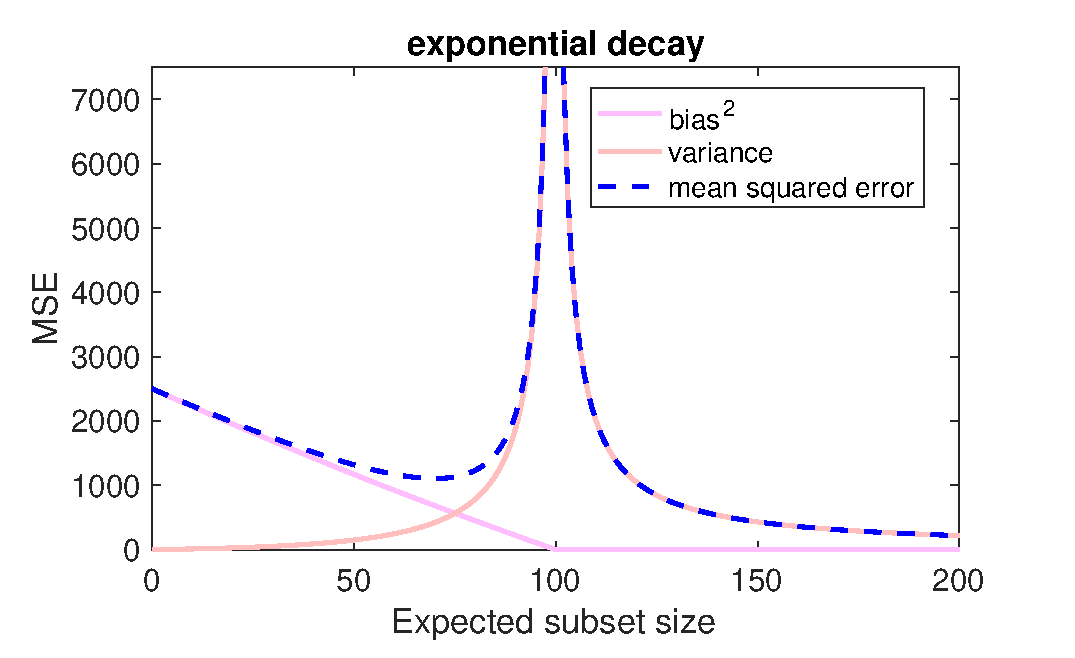
\includegraphics[width=0.49\textwidth]{figs/double-descent-primal}
    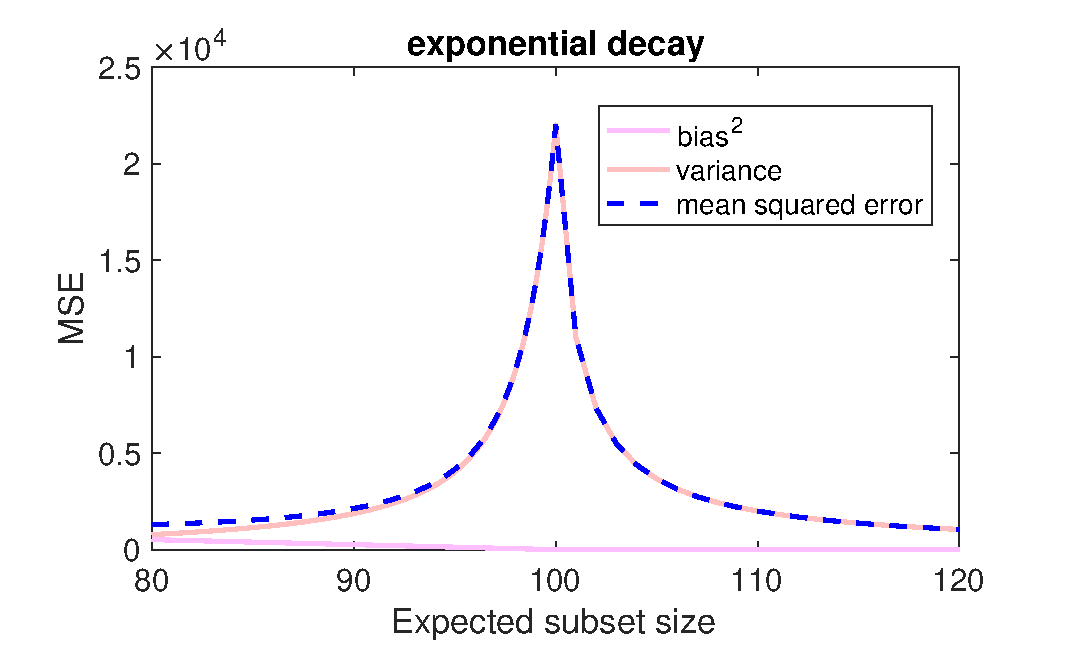
\includegraphics[width=0.49\textwidth]{figs/double-descent-primal-peak}
  \caption{Plot of the expressions from Theorem \ref{t:mse} and Remark
    \ref{r:sqinv} (sampling instances) against
    the expected subset size for a random $200\times 100$ matrix with
    exponentially decaying eigenvalues (left zooms in on the
    Y axis, right zooms in on the X axis).} 
\end{figure}
\paragraph{Next} Run experiments on real high-dimensional data by
averaging over multiple DPP samples.
\section{Sampling features}
Let $(\X,\y)$ be an $n\times d$ linear regression problem. We now
randomly select a subset of features $T\subseteq [d]$ and we predict
with the sparse
minimum-norm (when $|T|\geq n$) or least-squares (when $|T|< n$)
estimator: $\wbh_T = (\X\I_S)^\dagger\y$, where $^\dagger$ denotes 
the Moore-Penrose pseudoinverse and $\I_S=\sum_{i\in S}\e_i\e_i^\top$. 
% For the sake of consistency with our
% notation above, we let $\Z = \X^\top$ and use
\begin{theorem}
  If $T$ is sampled out of all subsets of $[d]$ so that $\Pr(T)\propto 
  \det(\frac1\lambda\X_{:,T}^\top\X_{:,T})$, then $\wbh_T$ is an unbiased
  estimator of the full ridge estimator with parameter $\lambda$, i.e.:
  \begin{align*}
    \E\big[\wbh_T\big] = (\X^\top\X+\lambda\I)^{-1}\X^\top\y.
  \end{align*}
\end{theorem}
\begin{theorem}\label{t:mspe-dual}
  Let $\X$ be an $n\times d$ matrix with columns in general
  position. Suppose that $\y=\X\w+\xib$, where
  $\xib\sim\Nc(\zero,\sigma^2\I)$. If $T\sim\Vol_\lambda(\X^\top)$, $k_\lambda=\E[|T|]$ and
  $\Sigmab_\lambda=(\X\X^\top+\lambda\I)^{-1}$, then:
  \begin{align*}
    \MSPE{\wbh_T}
    =\begin{cases}
    \sigma^2k_\lambda +
    (n-k_\lambda)\frac{\|\X\w\|^2_{\Sigmab_\lambda}}{\tr(\Sigmab_\lambda)},
    &\text{for }\lambda>0,\\
    \sigma^2n    &\text{for }\lambda\leq 0.
    \end{cases}
  \end{align*}
\end{theorem}
\begin{proof}
Let $\Z = \X^\top$. We will use the fact
that
\[\Z^\top(\Z^\top\I_T)^\dagger = \Z^\top\I_T\Z(\Z^\top\I_T\Z)^\dagger=
  \Z_T^\top\Z_T\Z_T^\dagger\Z_T^{\dagger\top}=\Z_T^\top\Z_T^{\dagger\top}= \Z_T^\dagger\Z_T,\]
which is a
projection matrix, and for $\lambda\leq 0$ we have $\Z_T^\dagger\Z_T=\I$.
\begin{align*}
  \MSPE{\wbh_T} &= \E\big[\|\Z^\top(\Z^\top\I_T)^\dagger\y - \Z^\top\w\|^2\big]\\
               &= \E\big[\|\Z_T^\dagger\Z_T(\Z^\top\w+\xib)-\Z^\top\w\|^2\big]\\
               &= \E\big[\|\Z_T^\dagger\Z_T\xib\|^2\big] +
                 \E\big[\|(\I-\Z_T^\dagger\Z_T)\Z^\top\w\|^2\big]\\
  &=\sigma^2\E\big[\tr(\Z_T^\dagger\Z_T)\big] +
    \E\big[\tr\big((\I-\Z_T^\dagger\Z_T)\Z^\top\w\w^\top\Z\big)\big]\\
(\text{for }\lambda>0)\quad  &=\sigma^2k_\lambda +
    \tr\big((\I+\tfrac1\lambda\Z^\top\Z)^{-1}\Z^\top\w\w^\top\Z\big)\\
  &=\sigma^2k_\lambda + \lambda\,\|\X\w\|^2_{(\X\X^\top+\lambda\I)^{-1}}.
\end{align*}
Note that $k = n-\lambda\, \tr\big((\X\X^\top+\lambda\I)^{-1}\big)$, so
the result follows.
\end{proof}

\begin{theorem}\label{t:mse-dual}
  Let $\X$ be an $n\times d$ matrix with columns in general
  position. Suppose that $\y=\X\w+\xib$, where
  $\xib\sim\Nc(\zero,\sigma^2\I)$. If $\Pr(T)\propto
  \det(\frac1\lambda\X_{:,T}^\top\X_{:,T})$, then:
  \begin{align*}
    \MSE{\wbh_T} &=
    \sigma^2\tr\big((\X\X^\top+\lambda\I)^{-1}\big)\bigg[1 +
    \frac{d-n}{n-d_\lambda}\Big(1-\frac{\det(\X\X^\top)}{\det(\X\X^\top+\lambda\I)}\Big)\bigg] &&\textnormal{variance}\\
    &\quad+\quad ???&&\textnormal{bias}^2
  \end{align*}
\end{theorem}
\Red{\bf It is not clear how to compute the bias. Previous proof had a mistake.}
\begin{proof}
Let $\Z = \X^\top$. Then we are sampling $T$ so that $\Pr(T)\propto\det(\frac1\lambda\Z_T\Z_T^\top)$.
\begin{align*}
  \MSE{\wbh_T} &= \E\big[\|(\Z^\top\I_T)^\dagger\y - \w\|^2\big]\\
               &= \E\big[\|(\Z^\top\I_T)^\dagger(\Z^\top\w+\xib)-\w\|^2\big]\\
               &= \E\big[\|(\Z^\top\I_T)^\dagger\xib\|^2\big] +
                 \E\big[\|(\I-(\Z^\top\I_T)^\dagger\Z^\top)\w\|^2\big].
\end{align*}
Note that $(\Z^\top\I_T)^\dagger = \I_T\Z(\Z_T^\top\Z_T)^\dagger$, so the variance part can be written as follows:
\begin{align*}
  \E\big[\|(\Z^\top\I_T)^\dagger\xib\|^2\big]
  &= \sigma^2\E\Big[\tr\big((\Z^\top\I_T)^\dagger (\Z^\top\I_T)^{\dagger\top}\big)\Big]\\
  &=
    \sigma^2\E\Big[\tr\big((\Z_T^\top\Z_T)^\dagger(\Z_T^\top\Z_T)^\dagger\Z_T^\top\Z_T\big)\Big]\\
  &=\sigma^2\E\Big[\tr\big((\Z_T^\top\Z_T)^\dagger\big)\Big]\\
  &=\sigma^2\bigg[\tr\big((\Z^\top\Z+\lambda\I)^{-1}\big) +
    \frac{(d-n)}{\lambda}\Big(1-\frac{\det(\Z^\top\Z)}{\det(\Z^\top\Z+\lambda\I)}\Big)\bigg]
\end{align*}
Next, we compute the bias term, letting $\bar T = [d]\backslash T$:
\begin{align*}
  \E\big[\|(\I-(\Z^\top\I_T)^\dagger\Z^\top)\w\|^2\big]
  &= \E\Big[\w^\top\big(\I - \Z(\I_T\Z)^\dagger\big)\big(\I-(\Z^\top\I_T)^\dagger\Z^\top\big)\w\Big]\\
  &= \|\w\|^2 - \E\big[2\,\w^\top\Z(\Z_T^\top\Z_T)^\dagger\Z^\top\I_T\w +
    \w^\top\Z(\Z_T^\top\Z_T)^\dagger\Z^\top(\I_T+\I_{\bar T})\w\big]\\
  &= \|\w\|^2 -
    \w^\top\Z\E\big[(\Z_T^\top\Z_T)^\dagger\Z^\top\I_T\big]\w +
    \w^\top\Z\E\big[(\Z_T^\top\Z_T)^\dagger\Z^\top\I_{\bar T}\big]\w\\
  &=\|\w\|^2 - \w^\top\Z\Z^\top(\lambda\I+\Z\Z^\top)^{-1}\w +
    \w^\top\Z\E\big[(\Z_T^\top\Z_T)^\dagger\Z^\top\I_{\bar T}\big]\w\\
  &=\lambda\,\w^\top(\X^\top\X+\lambda\I)^{-1}\w +
    \w^\top\Z\E\big[(\Z_T^\top\Z_T)^\dagger\Z^\top\I_{\bar T}\big]\w.
\end{align*}
% If $|T|< n$ and the rows of $\Z$ are in general position, then
% $(\Z_T^\top\Z_T)^\dagger\z_i=\zero$ for any $i\not\in T$. So
% \begin{align*}
%   \E\big[(\Z_T^\top\Z_T)^\dagger\Z^\top\I_{\bar T}\big]
%   &=
%   \Pr(|T|=n)\,\E\big[(\Z_T^\top\Z_T)^\dagger\Z^\top\I_{\bar T}\mid
%     |T|=n\big]\\
%   &= \frac{\det(\frac1\lambda\Z^\top\Z)}{\det(\frac1\lambda\Z^\top\Z+\I)}\,\E\big[(\Z_T^\top\Z_T)^{-1}\Z^\top -
%     (\Z_T^\top\Z_T)^{-1}\Z^\top\I_T\mid |T|=n\big]\\
%   &= \frac{\det(\Z^\top\Z)}{\det(\Z^\top\Z+\lambda\I)}\,\Big[(d-n+1)(\Z^\top\Z)^{-1}\Z^\top -
%     (\Z^\top\Z)^{-1}\Z^\top\Big]\\
%   &=\frac{\det(\Z^\top\Z) (d-n)}{\det(\Z^\top\Z+\lambda\I)} \,\Z^\dagger.
% \end{align*}
\end{proof}
\begin{theorem}\label{t:mse-dual-tail}
If we sample subset $T$ of fixed size $k\geq n$ so that $\Pr(T)\propto
  \det(\X_{:,T}\X_{:,T}^\top)$, i.e., volume sampling, then:
  \begin{align*}
    \MSE{\X_S^\dagger\y_S}
    &= \sigma^2\frac{d-n+1}{k-n+1}\tr\big((\X\X^\top)^{-1}\big)&&\textnormal{variance}\\
    &\quad+ \w^\top(\I-\X^\dagger\X)\w + \frac{d-k}{k-n+1}\w^\top\X^\dagger\X\w.&&\textnormal{bias}^2
  \end{align*}
\end{theorem}
% \begin{figure}[H]
%   \centering
%   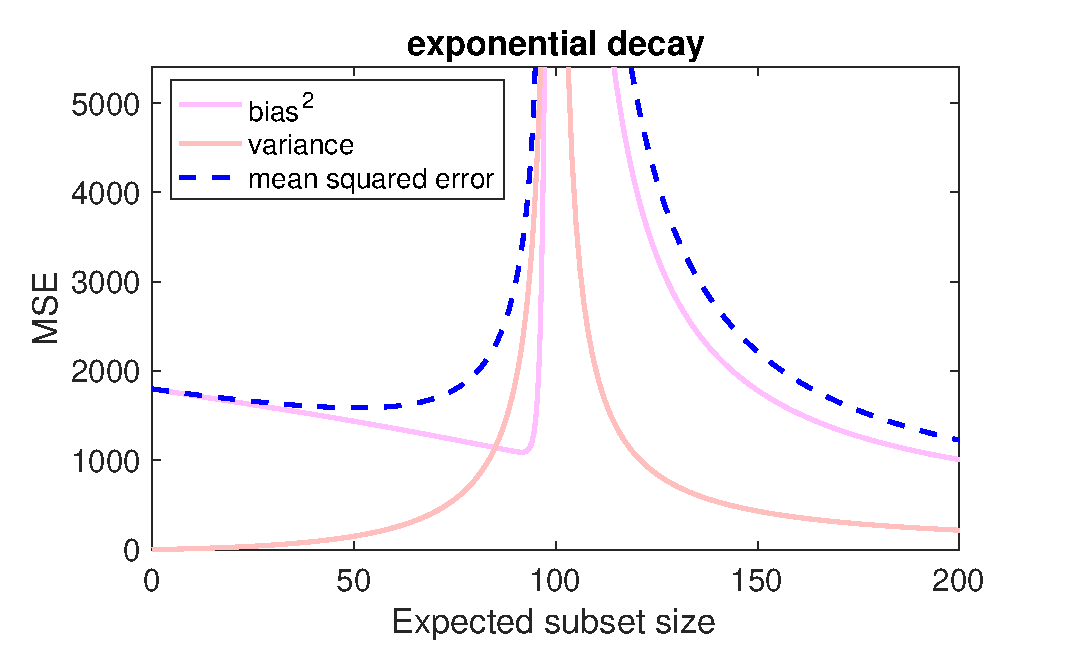
\includegraphics[width=0.49\textwidth]{figs/double-descent-dual}
%     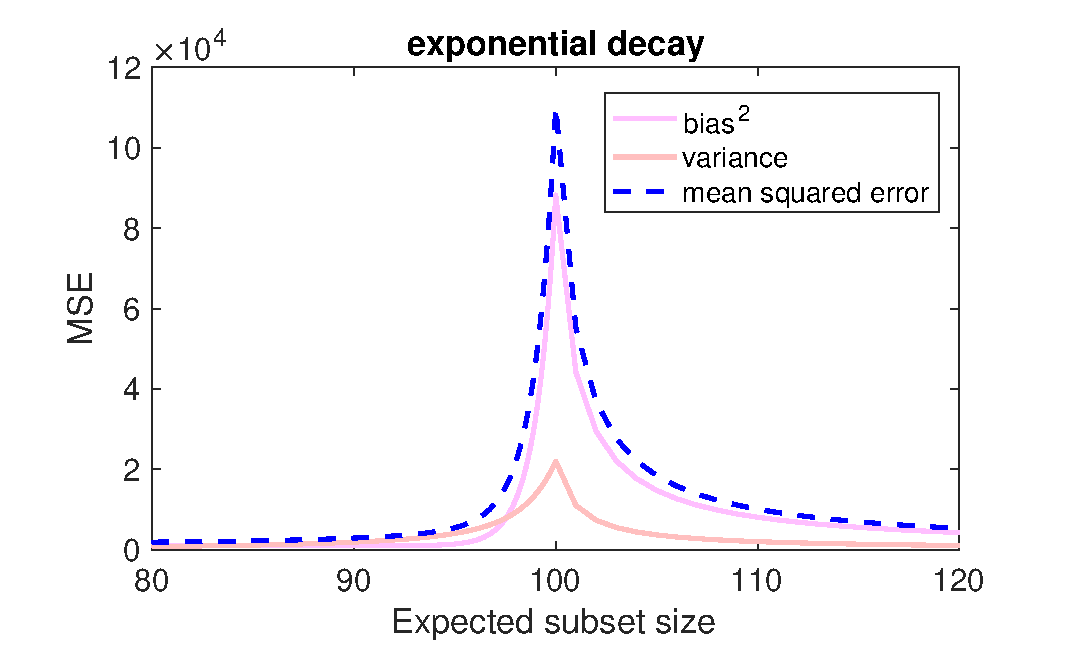
\includegraphics[width=0.49\textwidth]{figs/double-descent-dual-peak}
%   \caption{Plot of the expressions from Theorems \ref{t:mse-dual} and
%     \ref{t:mse-dual-tail} (sampling features)  against
%     the expected subset size for a random $100\times 200$ matrix with
%     exponentially decaying eigenvalues (left zooms in on the
%     Y axis, right zooms in on the X axis).} 
% \end{figure}

\section{Motivating DPPs as a model for feature selection}
Suppose that $\Z\in\R^{d\times n}$ is a population of feature vectors
($d$ rows of $\Z$). We may imagine that $d$ could be infinite, in
which case we would consider a distribution over features.
The task of a feature engineer is to select a set $S$ of $k$
features that will represent the population well. We propose the following model of a
feature engineer:
\begin{quote}
The \emph{oblivious feature engineer} does not have knowledge of the
population matrix $\Z$, however they 
can indicate their preference by defining a score function $f$ such that
$f(\Z_S)$ is a non-negative weight representing the believed quality
of a feature set $S$. The feature selection is realized by sampling
the set so that $\Pr(S)\propto f(\Z_S)$.
\end{quote}
Note that this idealized feature selection can be motivated by
considering a Markov chain procedure where we start with some subset
$S$ and then randomly pick two points $i\in S$ and $j\not\in S$ to
swap. We then accept the swap with probability
$\min\big\{1,\frac{f(\Z_{S-i+j})}{f(\Z_S)}\big\}$. The Markov chain
only requires a uniformly random access to features from $\Z$ and
converges to the distribution $\Pr(S)\propto
f(\Z_S)$. Note that this scheme requires us to fix the size
of the subset.

\textbf{Question:} What is the optimal score function for the
oblivious feature engineer? For now, we focus on the case of $k <
\min\{n,d\}$. One way to determine its quality is to ask how much 
 information do we lose by applying the orthogonal projection onto the
 subspace spanned by the features, $\P_{\!S}=\Z_S^\dagger\Z_S$, to the
 whole population matrix $\Z$. 
 We can evaluate this by looking at the sum of squares of the
 residuals: $\|\Z-\P_{\!S}\Z\|_F^2$.
The natural gold standard is top-$k$ PCA, which is the
best rank $k$ approximation of $\Z$, denoted $\Z_k$, and also a simple
example of an auto-encoder. Therefore, the \emph{value} of a score
function $f$ can be defined as:
\begin{align*}
  v_k(f) =  \max_{\Z}\frac{\E_{S\sim
  f\,:\,|S|=k}\big[\|\Z-\P_{\!S}\Z\|_F^2\big]}{\|\Z-\Z_k\|_F^2}. 
\end{align*}
\cite{pca-volume-sampling} showed that if
$f_{\DPP}(\Z_S)=\det(\Z_S\Z_S^\top)$, then $v_k(f)=k+1$. Also, they showed a
lower bound which says that for any $f$  we have $v_k(f)\geq
k+1$. This means that a cardinality constrained DPP is minimax optimal
in terms of $v_k$. Here are some further questions:
\begin{enumerate}
  \item Is the minimax optimal score function unique? In other words,
    can we show that for any $f\neq f_{\DPP}$ we have $v_k(f)>k+1$?
Simple first step, show that for $f$ uniformly equal $1$ we have
$v_k(f)=\infty$.
 \item The above requires that we fix the subset size, but we are
   actually analyzing a DPP with unconstrained size. Can we redefine
   the minimax value by replacing the cardinality constraint with an
   expected cardinality constraint? What is the minimax optimal score
   function then?
 \item The projection error is only well-defined for
   $k<\min\{n,d\}$. What is the natural way of extending this
   motivation to $k\geq \min\{n,d\}$? 
\end{enumerate}

\section{Tight analysis of the inverse formula}
Let $\pdet(\A)$ denote the pseudo-determinant of $\A$, i.e.,
the product of its non-zero eigenvalues.
\begin{theorem}
  Let $\X$ be an $n\times d$ matrix of rank $r$ whose rows are in
  general position within an $r$-dimensional subspace.
    If $S$ is sampled out of all subsets of $[n]$ so that $\Pr(S)\propto 
    \det(\X_S\X_S^\top)$, then
    \begin{align*}
    \E\big[(\I_S\X\X^\top\I_S)^\dagger\big] = (\I+\X\X^\top)^{-1} - \frac{\pdet(\X\X^\top)}{\det(\I+\X\X^\top)}\,(\I-\X^\dagger\X).  
    \end{align*}
  \end{theorem}
  \begin{remark}
    If $r= n$ then $\X^\dagger\X=\I$ and we get the
     formula: $\E\big[(\I_S\X\X^\top\I_S)^\dagger\big] = (\I+\X\X^\top)^{-1}$.
   \end{remark}
   \begin{proof}
     W.l.o.g.~assume that $r=d$.
     Let $\y\in\R^n$ be any vector. We will first compute
     \begin{align*}
       \det(\I+\X^\top\X)\,\E\big[\y^\top(\I_S\X\X^\top\I_S)^\dagger\y\big] =
       \sum_{S:|S|\leq d}\y_S^\top\adj(\X_S\X_S^\top)\y_S
     \end{align*}
     Each of those terms can be further simplified to:
  \begin{align*}
   \y_S^\top\adj(\X_S\X_S^\top)\y_S =
    \det(\X_S\X_S^\top+\y_S\y_S^\top) - \det(\X_S\X_S^\top)
    =\det\!\big([\X,\y]_S[\X,\y]_S^\top\big) - \det(\X_S\X_S^\top).
  \end{align*}
  Summing up over $S$ we obtain:
  \begin{align*}
    \sum_{S:|S|\leq d}\y_S^\top\adj(\X_S\X_S^\top)\y_S
    & =
    \sum_{S:|S|\leq d} \Big(\det\!\big([\X,\y]_S[\X,\y]_S^\top\big) -
\det(\X_S\X_S^\top)\Big) \\
&= \det\!\big(\I+[\X,\y][\X,\y]^\top\big) -\det(\I + \X\X^\top) -
\sum_{S:|S|=d+1}\det\!\big([\X,\y]_S[\X,\y]_S^\top\big) \\
&= \y^\top\!\adj(\I + \X\X^\top)\y -
\det\!\big([\X,\y]^\top[\X,\y]\big)\\
&=\det(\I+\X^\top\X)\,\y^\top(\I+\X\X^\top)^{-1}\y -
                                            \det(\X^\top\X)\,\y^\top(\I-\X^\dagger\X)\y.
  \end{align*}
  Since the formula holds for all $\y$'s, the result follows.
   \end{proof}

   \section{Square inverse formula for volume plus binomial sampling}
   \begin{theorem}\label{t:sqinv-binom}
     Let $\X$ be an $n\times d$ matrix whose rows are in general
     position. If $T\sim\Vol(\X)$ and $R\sim\mathrm{Bin}(n,p)$, then
     $S=T\cup R$ satisfies:
     \begin{align*}
       \E\big[(\X_S^\top\X_S)^{-1}\big] = (p\X^\top\X)^{-1}\cdot \big(1-(1-p)^{n-d+1}\big).
     \end{align*}
   \end{theorem}
   \begin{remark}
     If we set $p = \frac{k-d}{n-d}$ then $\E\big[|S|\big]=k$ and we get
\[     \E\big[(\X_S^\top\X_S)^{-1}\big] =
  \frac{n-d}{k-d}\,(\X^\top\X)^{-1}\cdot\bigg(1-\Big(\frac{n-k}{n-d}\Big)^{n-d+1}\bigg).\]
On the other hand, if we take $p\rightarrow 0$, then we recover
$\E\big[(\X^\top\X)^{-1}\big] = (n-d+1)\,(\X^\top\X)^{-1}$. 
\end{remark}
     \begin{proof}
       \begin{align*}
         \det(p\X^\top\X)&\,\E\big[(\X_S^\top\X_S)^{-1}\big]
         = \sum_{S}\det(\X_S^\top\X_S)(\X_S^\top\X_S)^{-1}p^{|S|}(1-p)^{n-|S|}\\
          &=
            \sum_{k=0}^n\sum_{S:|S|=k}\adj(\X_S^\top\X_S)p^k(1-p)^{n-k}
            \ - \sum_{S:|S|=d-1}\!\!\adj(\X_S^\top\X_S)p^{d-1}(1-p)^{n-d+1}\\
         &=\adj(p\X^\top\X) - \adj(\X^\top\X)p^{d-1}(1-p)^{n-d+1}\\
         &=\det(p\X^\top\X)(p\X^\top\X)^{-1}\big(1-(1-p)^{n-d+1}\big).
       \end{align*}
     \end{proof}
     \begin{corollary}
  Let $\X$ be an $n\times d$ matrix of rank $r$ whose rows are in
  general position within an $r$-dimensional subspace. If $T\sim\DPP(\X\X^\dagger)$ and $R\sim\mathrm{Bin}(n,p)$, then
  $S=T\cup R$ satisfies:
  \begin{align*}
    \E\big[\tr\big((\X_S^\top\X_S)^\dagger\big)\big] =
    \tr\big((p\X^\top\X)^\dagger\big)\cdot \big(1-(1-p)^{n-r+1}\big).
  \end{align*}
     \end{corollary}
     \begin{proof}
       Let $\L=\X\X^\top$. Since $\rank(\L)=r$, there is a matrix
       $\B\in\R^{n\times r}$ such that $\L=\B\B^\top$. It follows that
       $\DPP(\X\X^\dagger)=\Vol(\B)$. Moreover, since
       $\X_S\X_S^\top=\L_{S,S}=\B_S\B_S^\top$ for any $S\subseteq [n]$, we have
       \begin{align*}
         \tr\big((\X_S^\top\X_S)^\dagger\big) =
         \tr\big((\X_S\X_S^\top)^\dagger\big) =
         \tr\big((\B_S\B_S^\top)^\dagger\big) = \tr\big((\B_S^\top\B_S)^{-1}\big).
       \end{align*}
       In particular, we also have $\tr\big((\X^\top\X)^\dagger\big) =
       \tr\big((\B^\top\B)^{-1}\big)$. The result now follows by
       applying Theorem \ref{t:sqinv-binom}.
     \end{proof}

\section{Proof of Theorem \ref{t:unbiased}}
   \begin{proofof}{Theorem}{\ref{t:unbiased}}
Assume that $S\sim\DPP(\X\X^\top)$ (we can drop the $\lambda$
w.l.o.g.).  Let $\z\in\R^{d}$ be any vector. We will compute 
     \begin{align*}
       \det(\I+\X^\top\X)\,\z^\top\E\big[\X_S^\dagger\y_S\big] =
       \sum_{S:|S|\leq
       d}\det(\X_S\X_S^\top)\z^\top\X_S^\top(\X_S\X_S^\top)^{-1}\y_S
       =
\sum_{S:|S|\leq
       d}\z^\top\X_S^\top\adj(\X_S\X_S^\top)\y_S
     \end{align*}
     Each of those terms can be further simplified to:
  \begin{align*}
\z^\top\X_S^\top\adj(\X_S\X_S^\top)\y_S =
    \det(\X_S\X_S^\top+\y_S\z^\top\X_S^\top) - \det(\X_S\X_S^\top)
    =\det\!\big([\X,\y]_S[\X,\X\z]_S^\top\big) - \det(\X_S\X_S^\top).
  \end{align*}
  Summing up over $S$ we obtain:
  \begin{align*}
    \sum_{S:|S|\leq d}\z^\top\X^\top\adj(\X_S\X_S^\top)\y_S
    & =
    \sum_{S:|S|\leq d} \Big(\det\!\big([\X,\y]_S[\X, \X\z]_S^\top\big) -
\det(\X_S\X_S^\top)\Big) \\
&= \det\!\big(\I+[\X,\y][\X, \X\z]^\top\big) -\det(\I + \X\X^\top)\\
&= \z^\top\X^\top\!\adj(\I + \X\X^\top)\y \\
    &=\det(\I+\X\X^\top)\,\z^\top\X^\top(\I+\X\X^\top)^{-1}\y\\
    &=\det(\I+\X^\top\X)\,\z^\top(\I+\X^\top\X)^{-1}\X^\top\y.
  \end{align*}
  Since the formula holds for all $\z$'s, the result follows.
   \end{proofof}

\bibliography{pap}

   
\end{document}